\section{Procurement Simulation}
\label{procuresim}
The procurement simulation represents the marketplace for suppliers, so  the place where the player can buy the components needed for producing the products. In the UI the procurement view is also referred to as harbour. At the marketplace the player can also buy the retail products, whereas the buying process works the same way as for the products that need to be manufactured. However, the retail products are not part of the current prototype implementation.

In order to be able to produce a product, the player needs all the required components of a certain product. For example, he would need exactly one component (\gls{c}) out of the following \textit{componentCategories}, to produce a smartphone: Power supply , display and case, CPU, camera, connectivity. Moreover, each \textit{componentCategory} has different levels, such as the "camera", which has the levels "1.2 MP", "2 MP", "5 MP", "8 MP" and "12 MP".  As soon as the player chooses to produce a new smartphone, the first level of a component is selected. For the component "camera" this would be the level "1.2 MP". However, the camera component would not be unlocked until the first level of the camera component is activated. For the camera component this would be the year 2004. This behavior will be explained in more detail later in this chapter.

Moreover, it is possible to manufacture more than one product in a product category in order to test the market. For example, the player could produce two smartphones, one made of cheap components and with a low \textit{salesPrice}, and one made of expensive components with a higher \textit{salesPrice}. Additionally, the player can specify the name of a product to distinguish it from the others and he can add and remove products from his product portfolio.

Furthermore, the different levels of a component are considered as individual components and one supplier for each \textit{supplierCategory} (premium, regular, cheap) is offered. This results in three different suppliers for each individual component.\\
Apart from that, each individual component has the following attributes:
\begin{itemize}
    \item componentCatgeory
    \item componentName
    \item componentLevel
    \item initialComponentPrice
    \item supplierCategory
    \item baseCost
    \item supplierQuality
    \item supplierEcoIndex
    \item baseUtility
    \item availabilityDate
\end{itemize}
Each of these attributes fulfills a specific need. For example, the \textit{baseCost} of a component, which represents a components purchase price offered by one supplier, depends (not linearly) on the \textit{supplierQuality} and the \textit{supplierEcoIndex}. This is achieved by the settings shown in table \ref{component_price_calculation}.
    \begin{table}[ht]
    \centering
    \begin{tabular}{|l|r|r|r|}
    \hline
    supplierCategory & supplierCostMultiplicator & supplierQuality & supplierEcoIndex \\
    \hline
    premium & 1.1 - 1.5 & 80 - 100\% & 80 - 100\% \\
    regular & 0.85 - 1.2 & 55 - 85\% & 55 - 85\%\\
    cheap  & 0.7 - 1.0 & 10 - 60\% & 10 - 60\%\\
    \hline
    \end{tabular}
    \caption{Randomized value ranges for the calculation of baseCost, supplierQuality and supplierEcoIndex}
    \label{component_price_calculation}
    \end{table}
\newline
The three factors (\textit{supplierCostMultiplicator, supplierQuality, supplierEcoIndex}) shown in table \ref{component_price_calculation} are randomized within a specific value range. That helps to break up static pricing behavior and make the game more interesting. In addition, the value ranges of the three different \textit{supplierCategories} (premium, regular, cheap) overlap. This increases the degree of difficulty for the user, as this could lead to a "regular" component having a better \textit{baseCost-supplierQuality-supplierEcoIndex} trade-off than a "premium" component. 

The \textit{baseCost} of a component is calculated by multiplying the \textit{timeBasedComponentPrice} (\gls{tBCP}) with the \textit{supplierCostMultiplicator} as shown in equation \ref{baseCost}.
\begin{equation}
\label{baseCost}
\begin{aligned}
   baseCost_{c} = tBCP_{c} \cdot supplierCostMultiplicator
\end{aligned}    
\end{equation}

The \textit{timeBasedComponentPrice} is the calculated price of a component that is based on the \textit{initialComponentPrice} and depends on a component's \textit{availabilityDate}. The \textit{availabilityDate} is required to activate a \textit{componentLevel}. This means that a particular level of a component is activated when it reaches the year in which it is released, as it is locked before exceeding its \textit{availabilityDate}. In summary, the use of the \textit{availabilityDate} ensures that the player cannot directly select the latest level of a component, but is bound to the chronological development of the components.

Moreover, a component's \textit{ecoIndex} and \textit{supplierQuality} are calculated by selecting a random integer value within the defined value range. An example of determining the \textit{supplierEcoIndex} of a "premium" component is shown in equation \ref{supplierEcoIndex}.
\begin{equation}
\label{supplierEcoIndex}
    supplierEcoIndex_{c}(premium \; component) = randomized(80-100)
\end{equation}

Furthermore, each component has a \textit{baseUtility}, which is defined manually. This is the case because the changes of the \textit{baseUtility} differ greatly between the different versions of a component. For example, for cameras, the increase in \textit{baseUtility} from the first level to the second level, from "1.2 MP" to "2 MP", is much lower than the increase from the second to the third level, from "2 MP" to "5 MP".

The \textit{supplierEcoIndex}, \textit{supplierQuality} and \textit{baseUtility} represent the variables needed for the calculation of the \textit{totalProcurementQuality} (\gls{tProcureQ}) per product, which is shown in equation \ref{totalProcurementQuality}. The \textit{totalProcurementQuality} then influences the \textit{totalProductQuality} of a product.
\begin{equation}
\label{totalProcurementQuality}
\begin{aligned}
    tProcureQ_{p}= \sum_{c \in C_p} & (0.4 \cdot supplierEcoIndex_{c} + 0.6 \cdot supplierQuality_{c})\\
    & \cdot ~baseUtility_{c}
    \end{aligned}
\end{equation}

All components (\textit{componentCategories}) per product (\textit{productCategory}) including their static attributes, which are \textit{componentLevel}, \textit{componentName}, \textit{availabilityDate} and \textit{baseUtility}, can be found in appendix \ref{fig:staticComponentAttributes}.\\
Figure \ref{img:totalComponentCosts} should help to understand the complex calculation of a component's \textit{baseCost}, as well as the relation and the influences between the different attributes of a component and a component’s initial price (\textit{initialComponentPrice}).

\begin{figure} [H]
	\centering
	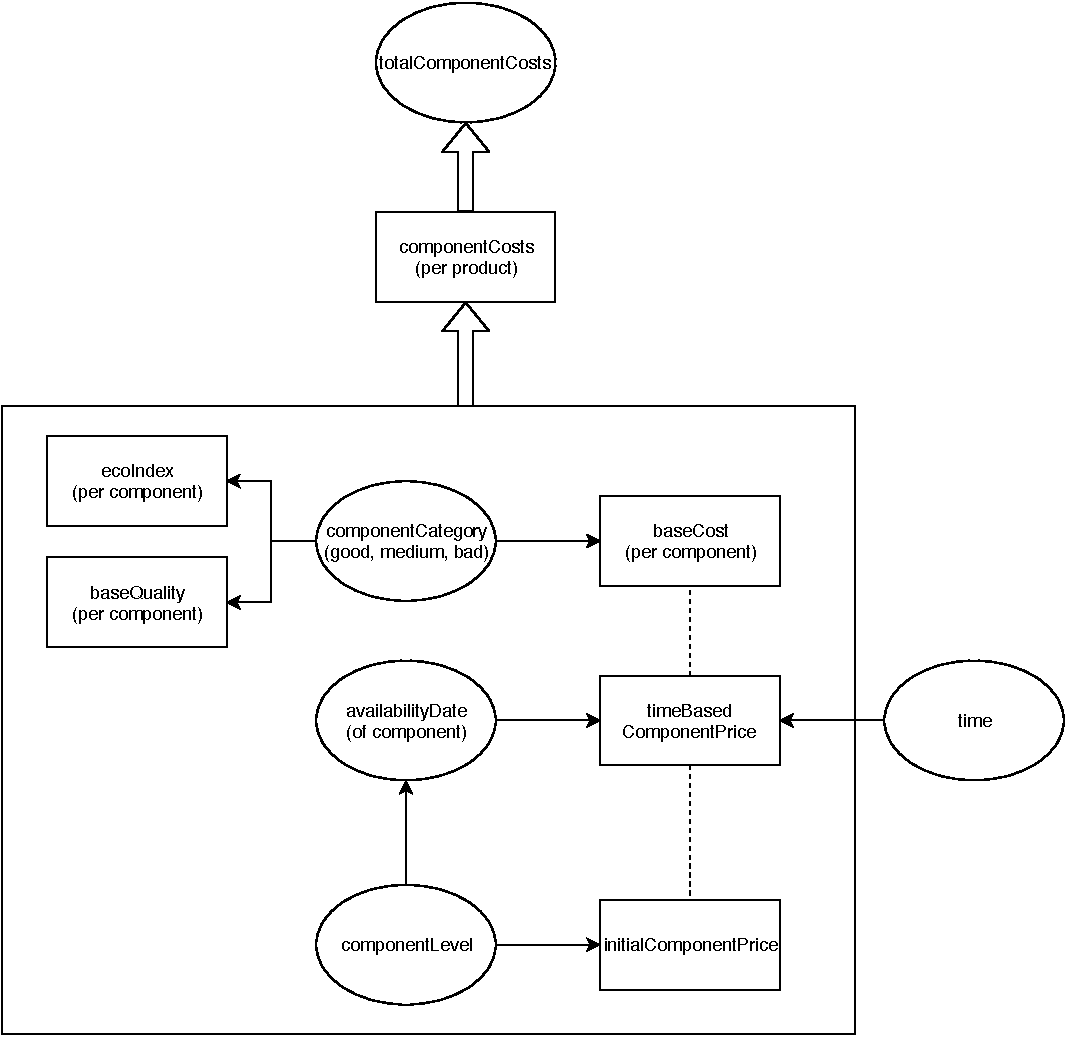
\includegraphics[width=11.5cm]{images/totalComponentCosts.pdf}
	\caption{Composition of \textit{totalComponentCosts}}
	\label{img:totalComponentCosts}
\end{figure}

Starting from the bottom of figure \ref{img:totalComponentCosts}, the \textit{initialComponentPrice} is available for each component and depends on the \textit{componentLevel}.
The \textit{timeBasedComponentPrice} depends on the \textit{time}, on the \textit{availabilityDate} of a component, and on the \textit{initialComponentPrice}, which in turn depends on the \textit{componentLevel}.
The \textit{timeBasedComponentPrice} is dependent on the \textit{time} because we assume that a supplier produces a component in a certain level for a certain amount of time. In the first year, this is then state-of-the-art technology. However, as state-of-the-art technology rapidly become outdated and additionally new \textit{componentLevels} are released, the \textit{timeBasedComponentPrice} decreases starting from the second year on.

The \textit{timeBasedComponentPrice} is calculated by multiplying the \textit{initialComponentPrice} with the \textit{timeBasedPriceMultiplicator} (tBPM), as shown in equation \ref{Function timeBasedComponentPrice}. The \textit{timeBasedPriceMultiplicator} in turn is calculated according to the polynomic function \ref{Function timeBasedPriceMultiplicator} of fifth degree, which was interpolated from component values loosely based on historical component prices found on multiple Internet sources such as \href{https://camelcamelcamel.com}{camelcamelcamel.com}.
\begin{equation}
\label{Function timeBasedPriceMultiplicator}
\begin{aligned}
   tBPM_{c}(t_y, c) = & - 0.0001(t_y-availabilityDate_{c}+1)^5 \\
   & - 0.0112(t_y-availabilityDate_{c}+1)^4 \\
   & - 0.4239(t_y-availabilityDate_{c}+1)^3 \\
   & + 7.3219(t_y-availabilityDate_{c}+1)^2 \\
   & - 49.698(t_y-availabilityDate_{c}+1) \\
   & + 142.7889 &&
\end{aligned}   
\end{equation}
\begin{equation}
\label{Function timeBasedComponentPrice}
    tBCP_{c} (iCP, tBPM) = iCP \cdot \dfrac{tBPM}{100}
\end{equation}

\begin{figure} [H]
    \centering
	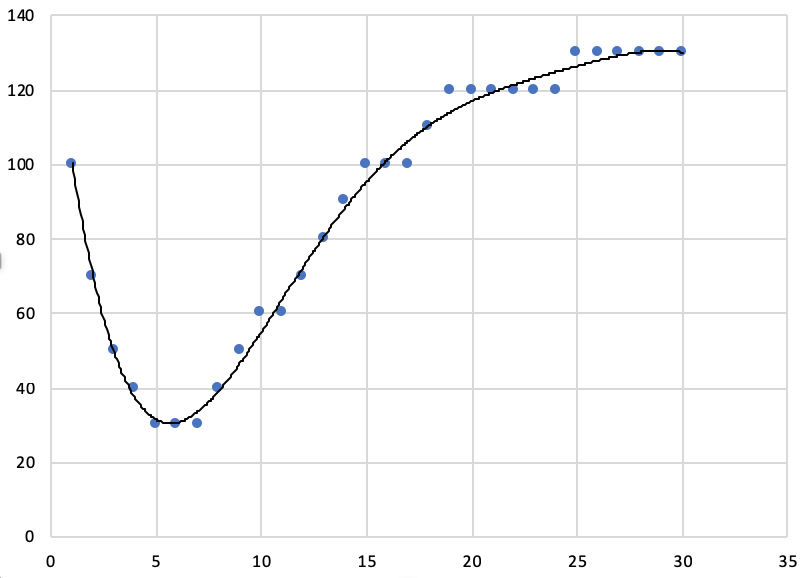
\includegraphics[width=9.5cm]{images/timeBasedComponentFunction.png}
	\caption{Function of \textit{timeBasedComponentPrice}}
	\label{img:timeBasedComponentPriceFunction}
\end{figure}
As it can be seen in picture \ref{img:timeBasedComponentPriceFunction} the \textit{timeBasedComponentPrice} decreases until the 5th year, stays stable for a short while on this reduced level, and then starts increasing again. The increase is due to the assumption that a supplier will discontinue the production of a component with a certain \textit{componentLevel} after some time because a newer level is released or available on the market. Since the supplier’s stock could be empty at this point, the component becomes a rarity. Therefore the component becomes more expensive compared to its \textit{initialComponentPrice}.\\
Afterwards, based on the \textit{timeBasedComponentPrice} and the \textit{supplierCategory} (which can either be premium, regular or cheap) a component's \textit{baseCost} is calculated. Moreover, also a component's \textit{supplierEcoIndex} and \textit{supplierQuality} depend on the \textit{supplierCategory}.\\
The \textit{componentCosts} per product can then be calculated by adding up the \textit{baseCost} of the selected components per product. All \textit{componentCosts} together then determine the \textit{totalComponentCosts} of all produced products.\\

In the following, further ideas for the procurement simulation are explained which have not yet been implemented or tested in our prototype, but which are also part of our concept.

A volume discount would allow the player to get a 10 percent discount, for example, if he buys more than 300 units of a component. We postponed this idea because our prototype does not include units in the procurement simulation yet. Currently, the player only needs to select a component and it is assumed that the desired quantity is delivered for just-in-time production. 
The aim, however, is to leave the purchase decision to the user, who would have to calculate the trade-off between the benefits of lower prices per component due to volume discounts and higher storage costs for storing all non-producible components.